\section{Methodology}\label{sec:methodology}


\subsection{SUMO and TraCI}
\tech is evaluated in the simulator SUMO (Simulation of Urban Mobility)\cite{sumo} interfaced via TraCI (Traffic Control Interface)\cite{traci}.
SUMO is a large-scale open source project rooted in the institute of Transportation Systems at the German Aerospace Center.
SUMO is a microscopic simulator, that models individual vehicles, detailed road networks and traffic lights as explained in Section~\ref{sec:Model}.

As SUMO is a microscopic simulator it imposes a number of restrictions and simplifications.
No vehicle may drive above the maximum speed of the road, acceleration and deceleration is a constant value independent of the speed, no vehicle can drive into other vehicles, vehicles always waits for blocking traffic, but they do not show consideration for others and wait if someone needs to change lanes.
This last fact introduces a dead lock problem.
If an area has a high congestion, two vehicles might end up waiting to change to into each others lanes, but at the same time blocking the other vehicle in doing so. 
SUMO handles this problem by eventually teleporting the vehicles along the network until they can be reinserted. 
This is often just at the opposite side of the traffic light.

SUMO has a build-in function to calculate the vehicles fuel consumption, which is explained in \cite{SUMOFuel}.
This function is used to estimate the reduction in fuel consumption.

\subsection{Use Case}\label{sec:UseCase}
%Best guess configuration
We evaluate \tech on a frequently used section of Hobrovej in Aalborg, Denmark (See Figure~\ref{fig:Introduction:hobro}).
The simulations should be as realistic as possible and therefore based on real data. 
The road network should have the same dimensions, the traffic signals should behave similar and the congestion levels should be similar to what is observed in the real world.

The section has seven junctions: two large regulated junctions with $12$ to $16$ connections, two small regulated junctions with $4$ to $6$ connections, and three small unregulated junctions.
The network is an exact replica of Hobrovej, with the same distance between segments and the same number of lanes and connections.
We will many focus on the route going from the south end of Hobrovej to the north end of Hobrovej.
\begin{figure}[htb]
\centering
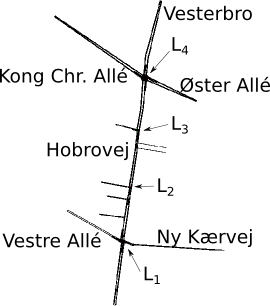
\includegraphics[width=0.3\textwidth]{../images/HobrovejNy.png}
\caption{Road network}
\label{fig:Introduction:hobro}
\end{figure}

We have estimated the phases of traffic lights based on local knowledge of the area and a circulation time of 100 seconds.
The number of routes and vehicles in the network is also based on local knowledge of the area and an OD (Origin-Destination) matrix extracted from GPS trajectories from the project "Spar På Farten"\cite{SparPaFarten}.
Each simulation has $2362$ vehicles spawning on a random route, keeping with the values of the OD matix.
The spawn rate is defined as the number of vehicles entering the network per second.
To evaluate \tech at different levels of congestion, we run the tests with different spawn rates ranging from $0.4$ to $1.8$ vehicles per second.
At each congestion level, we run the simulation four times with 0\%, 10\%, 50\%, 100\% vehicles using the system.
Initially, we will focus on the tests with a spawn rate of $0.8$ vehicle per second. %TODO:  check this 0.8
This corresponds to the average congestion in the daytime outside peak loads on the primary route in the network.

We only model vehicles of the types detailed in Tabel~\ref{table.vehicleTypes}, and do not model neither pedestrians nor cyclists.
The maximum speed on the network is $60km/h$ which was the speed limit when the data from "Spar På Farten" was collected.
In the evaluations, we only use one type of vehicle, detailed in Table~\ref{table.vehicleTypes}. 
All values are based on common knowledge and the GPS trajectories from "Spar På Farten".

\begin{table}
\centering
\begin{tabular}{|l|l|l|}\hline
Acceleration			& $1.9 m/s^2$	\\\hline
Deceleration			& $3 m/s^2$ 	\\\hline
Length					& $4 m$ 		\\\hline
Maximum speed			& $41 m/s \sim 147.6 km/h$ \\\hline
Min. gap to vehicles	& $2 m$ 		\\\hline
\end{tabular}
\caption{Vehicle specification}\label{table.vehicleTypes}
\end{table}



